% Revised system and interaction design preprint (2026-10-16)
% This is an independent preprint, NOT an ACM or Springer proceedings PDF.
% The preliminary workshop listing refers to an earlier version.
% Build: latexmk -pdf -interaction=nonstopmode -halt-on-error main.tex
% Figure 1 is drawn in TikZ and Figure 2 is an actual local UI Preview screenshot.
% No controlled study, model benchmark, or validated end-to-end source navigation is claimed.
\documentclass[manuscript,screen,nonacm]{acmart}
\usepackage{booktabs}
\usepackage{tabularx}
\usepackage{array}
\usepackage{tikz}
\usetikzlibrary{arrows.meta,positioning}
\settopmatter{printacmref=false,printccs=false}
\setcopyright{none}
\hypersetup{hidelinks,pdfauthor={Rongyu Wang},pdfsubject={Revised system and interaction-design preprint, 16 October 2026},pdfkeywords={Multimodal RAG, Human-AI Interaction, Evidence Provenance, Temporal Navigation, Verifiable Interaction}}
\graphicspath{{./}}
\urlstyle{same}

\title{Designing Temporally Grounded Multimodal Learning Interfaces for Verifiable Interaction}
\author{Rongyu Wang}
\affiliation{\institution{University of Reading}\city{Reading}\country{United Kingdom}}
\email{rongyu.wang@student.reading.ac.uk}

\begin{abstract}
Textbooks, diagrams, and recorded lectures often provide complementary accounts of the same concept. Conversational learning assistants can retrieve relevant material, yet learners still need a way to inspect the original source of a generated statement. We present a system and interaction design for a multimodal retrieval-augmented learning prototype that indexes textbook passages, descriptions of textbook figures, and timestamped descriptions of sampled lecture-video frames. The principal design contribution is a \emph{provenance-to-viewer mapping}: retrieved records retain document-page or video-time information that can be resolved into inspectable source actions through an explicit local source registry. We report the implementation boundary of a public Python/Streamlit prototype, including dense retrieval, an evidence-first split-pane interface, structured evidence controls, and missing-source states. Speech transcription, sparse lexical retrieval, automatic claim-level attribution, and validated end-to-end source navigation are not established by the available implementation evidence. We call the intended interaction \emph{verifiable interaction}: moving from a generated explanation or retrieved reference to a source the learner can inspect. This is a system and interaction-design account, not an evaluation of retrieval accuracy, interface usability, or learning outcomes.
\end{abstract}
\keywords{Multimodal RAG, Human--AI Interaction, Learning Interfaces, Evidence Provenance, Temporal Navigation, Verifiable Interaction}

\begin{document}
\maketitle
\noindent{\footnotesize\textit{Version and availability.} Revised system and interaction-design preprint, 16 October 2026. A preliminary version was listed in the \emph{Spotlight Presentations II} session of the AIED 2026 Workshop on Designing and Evaluating Next-Generation Learning Interfaces (\url{https://extendedhorizon.com/aied2026ws-ai-hci-ls/program/}). This revision has not been claimed as a separate peer-reviewed or proceedings publication. Accompanying public code: \url{https://github.com/William-Turing/multimodal-rag-verifiable-tutor} (initial public commit \texttt{1254e87}).}\par

\section{Introduction}
Educational materials rarely exist in one modality. A textbook may define a concept, a figure may illustrate its structure, and a recorded lecture may demonstrate an example. Learners must often move between document search, video playback, and their own notes to connect these sources. A conversational assistant reduces the effort of asking an initial question, but a plausible answer without an actionable source reference is difficult to assess.

Retrieval-augmented generation (RAG) conditions language generation on retrieved material~\cite{lewis2020rag}. Multimodal RAG investigates retrieval and generation over representations beyond ordinary text~\cite{hu2025mrag}. Neither approach, by itself, guarantees that a learner can reach the passage or lecture moment on which an answer appears to rely. We distinguish \emph{retrieving a candidate record} from \emph{making its provenance actionable}.

Our design question is: \emph{How can a multimodal learning interface make the provenance of AI-generated responses inspectable across textbooks and lecture videos?} The organizing interaction is \emph{claim $\rightarrow$ evidence reference $\rightarrow$ original source $\rightarrow$ learner inspection}. This loop is a design objective, not a verified claim-by-claim reasoning trace.

This paper makes three contributions: (1) a multimodal learning-interface architecture coupling retrievable text and visual descriptions with source-location metadata; (2) a provenance-to-navigation interaction specification, with an implementation account of source resolution and failure handling; and (3) a design analysis clarifying what source inspectability can and cannot establish. The newly available source-code artifact lets us distinguish implemented mechanisms from design intentions rather than relying on an earlier interface screenshot alone.

\section{Related Work}
\subsection{Multimodal RAG and Educational AI}
RAG combines retrieved external information with generation~\cite{lewis2020rag}. Multimodal RAG studies how different kinds of content can be represented and retrieved~\cite{hu2025mrag}. Dela Rosa~\cite{delarosa2025video} describes video retrieval with aligned captions, while MDKAG~\cite{zhao2025mdkag} organizes educational question answering through a multimodal disciplinary knowledge graph. These lines of work motivate using multiple evidence representations. Our emphasis is more specific: retaining source locations and turning retrieved-record provenance into source-inspection controls.

\subsection{Temporal Navigation and Learning}
Multimedia-learning research examines the joint presentation of verbal and visual material~\cite{mayer2020multimedia}. Video question-answering research addresses temporal and visual reasoning~\cite{zhong2022video}. A timestamp has a narrower function in the present prototype: it can identify a requested playback location. Addressable time metadata is not proof that the correct instructional event was found.

\subsection{Inspectable Human--AI Interfaces}
Guidelines for human--AI interaction emphasize communication of capabilities, graceful failure, and appropriate reliance~\cite{amershi2019guidelines}. Explanations also need to be evaluated in relation to their human audience~\cite{miller2019explanation}. A source link is not an explanation of a model's internal reasoning; it offers an opportunity to compare generated language with an external document or recording. Epistemic vigilance~\cite{sperber2010vigilance} and self-regulated learning~\cite{zimmerman2002self} provide theoretical motivation for such inspection, not evidence that users will always perform it. Broader opportunities and risks for educational language models have also been documented~\cite{kasneci2023chatgpt}.

\section{System and Interface Design}
\subsection{Design Goals and Scope}
We distinguish four design goals: \textbf{G1} represent textbook text, textbook figures, and sampled lecture-video frames as searchable records; \textbf{G2} preserve source identity and available page or time coordinates; \textbf{G3} make retrieved references actionable within an evidence workspace; and \textbf{G4} support evidence-aware conversational guidance while preserving the option to inspect original material. These goals are not measured learning achievements. A speech-transcript retrieval path remains a proposed extension rather than an implemented component of the current public code.

\begin{figure}[t]
\centering
\resizebox{0.98\linewidth}{!}{%
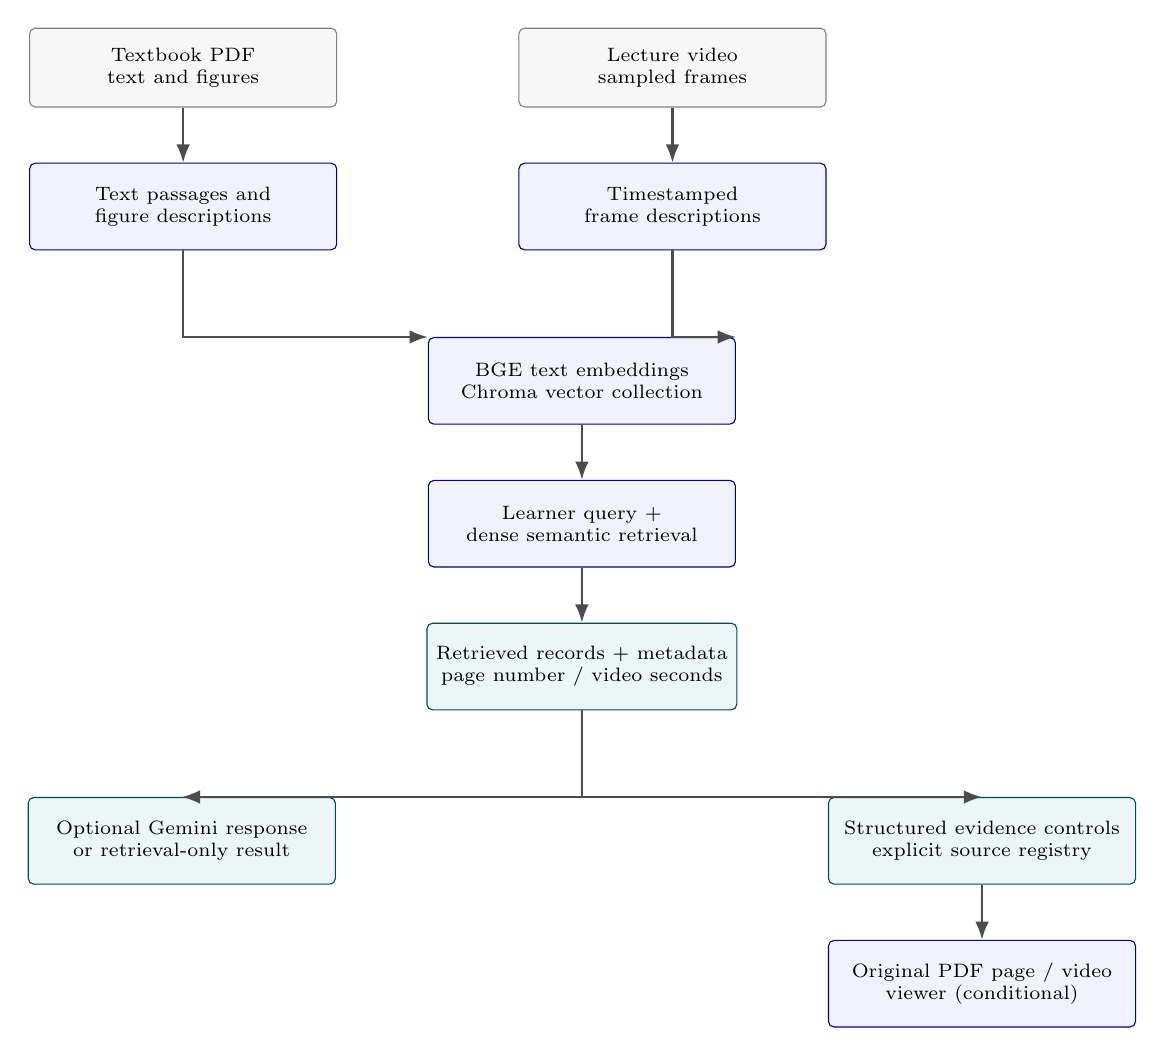
\begin{tikzpicture}[
  node distance=7mm and 11mm,
  >=Latex,
  input/.style={draw=black!50, rounded corners=2pt, fill=black!3, minimum width=39mm, minimum height=10mm, align=center, font=\scriptsize},
  process/.style={draw=blue!55!black, rounded corners=2pt, fill=blue!5, minimum width=39mm, minimum height=11mm, align=center, font=\scriptsize},
  evidence/.style={draw=teal!60!black, rounded corners=2pt, fill=teal!7, minimum width=39mm, minimum height=11mm, align=center, font=\scriptsize},
  optional/.style={draw=black!50, rounded corners=2pt, dashed, fill=black!1, minimum width=35mm, minimum height=11mm, align=center, font=\scriptsize},
  line/.style={->, thick, draw=black!70}
]
\node[input] (pdf) {Textbook PDF\\text and figures};
\node[input, right=23mm of pdf] (video) {Lecture video\\sampled frames};
\node[process, below=of pdf] (pdfp) {Text passages and\\figure descriptions};
\node[process, below=of video] (vidp) {Timestamped\\frame descriptions};
\node[process, below right=11mm and 11.5mm of pdfp] (index) {BGE text embeddings\\Chroma vector collection};
\node[process, below=of index] (retrieval) {Learner query +\\dense semantic retrieval};
\node[evidence, below=of retrieval] (record) {Retrieved records + metadata\\page number / video seconds};
\node[evidence, below left=11mm and 11.5mm of record] (answer) {Optional Gemini response\\or retrieval-only result};
\node[evidence, below right=11mm and 11.5mm of record] (chip) {Structured evidence controls\\explicit source registry};
\node[process, below=of chip] (viewer) {Original PDF page / video\\viewer (conditional)};
\draw[line] (pdf)--(pdfp);
\draw[line] (video)--(vidp);
\draw[line] (pdfp.south) |- (index.north west);
\draw[line] (vidp.south) |- (index.north east);
\draw[line] (index)--(retrieval);
\draw[line] (retrieval)--(record);
\draw[line] (record.south) |- (answer.north);
\draw[line] (record.south) |- (chip.north);
\draw[line] (chip)--(viewer);
\end{tikzpicture}%
}
\Description{Implementation-oriented architecture diagram. Textbook passages and figure descriptions and timestamped lecture-frame descriptions are embedded into a Chroma dense-vector collection. Retrieved nodes retain metadata and can be passed separately to optional answer generation and structured source controls. A source registry conditionally resolves source-viewer actions.}
\caption{Implementation-oriented architecture. Solid arrows represent code paths represented in the public repository; a successful complete live run is not implied. Audio transcription, BM25/sparse retrieval, and claim-level attribution are not shown because they are not implemented in the audited code.}
\label{fig:architecture}
\end{figure}

\subsection{Multimodal Ingestion}
Figure~\ref{fig:architecture} summarizes the auditable implementation paths. The PDF processor uses PyMuPDF to extract page text and LlamaIndex \texttt{SentenceSplitter} to produce retrievable passages with one-based \texttt{page\_number} metadata. An optional figure-processing path extracts suitable raster images and obtains textual descriptions using a vision-capable Gemini model. These descriptions support text-based retrieval; they are not direct image embeddings and need not preserve all information in the original diagram.

The video processor samples frames using OpenCV and a scene-change heuristic, then requests frame descriptions from Gemini. Its exported records contain seconds, a readable timestamp, and a textual description. This path processes visible frame content; it does \emph{not} extract or transcribe speech. Consequently, we do not claim synchronized lecture transcripts, audio--visual alignment, or spoken-evidence search. Model-derived descriptions can omit, misread, or invent visual details, and sampling can miss short instructional events.

\subsection{Dense Retrieval and Provenance}
The prototype uses the \texttt{BAAI/bge-small-en-v1.5} text-embedding model with LlamaIndex and a persisted Chroma collection for dense semantic retrieval. A learner question retrieves up to six candidate records in the current application configuration. This description concerns the implemented retrieval path; no benchmark or relevance comparison is reported. Retrieval choices may also affect the quality of context supplied to generation~\cite{cuconasu2024noise}. The earlier workshop manuscript referred to lexical matching, but the public implementation does not contain a separately documented BM25 index, sparse retriever, or fusion stage. Hybrid retrieval is therefore not claimed.

A usable evidence reference requires both retrievable content and a source coordinate. Table~\ref{tab:provenance} separates the intended record-level provenance contract from optional future precision. A page number identifies a PDF page, not a highlighted sentence. A video timestamp requests a playback position, not a verified semantic alignment with a spoken explanation.

\begin{table}[t]
\caption{Provenance coordinates and intended navigation behavior. These are interface requirements, not automatically validated citations.}
\label{tab:provenance}
\small
\begin{tabularx}{\linewidth}{@{}>{\raggedright\arraybackslash}p{0.20\linewidth}>{\raggedright\arraybackslash}p{0.37\linewidth}X@{}}
\toprule
Record & Required / optional coordinates & Intended action \\
\midrule
PDF passage & Source identifier; page; optional passage geometry & Open the original PDF page; highlight only if trustworthy coordinates exist \\
Figure description & Source identifier; page if retained; original image reference if available & Open a verified source page / image, otherwise show an unavailable state \\
Video frame description & Source identifier; nonnegative time in seconds; optional keyframe or interval & Request player seek to the indexed time \\
Transcript segment (future) & Video identifier; speech interval; transcript text & Seek to speech interval if an ASR pipeline is added \\
\bottomrule
\end{tabularx}
\end{table}

\subsection{Evidence-Aware Response Generation}
The optional answer-generation step receives a learner question and retrieved text records. The current prompt asks Gemini to cite only provided evidence identifiers (for example, \texttt{[E1]}) and to avoid inventing page numbers or times. It can request a reflective question as conversational scaffolding. This prompting strategy does not guarantee evidence fidelity or educational appropriateness. Importantly, model-generated references in prose do not determine navigation: the clickable source controls are derived from the retrieved node's metadata. The application does \emph{not} automatically align or verify each generated sentence with a supporting passage.

\subsection{Evidence-First Interface and Citation Resolution}
The revised Streamlit interface places conversation beside an evidence workspace (Figure~\ref{fig:ui}). Retrieved-source buttons are associated with stored evidence objects; selection updates the active record and its metadata panel. The supporting source resolver consults an explicitly configured local \texttt{sources.json} registry. Where an indexed record contains a stable source identifier, resolution uses that identifier. For legacy nodes with generic labels such as \texttt{PDF Document} or \texttt{Video Tutorial}, an alias resolves only if it uniquely matches an explicitly configured source of the proper type. The resolver does not guess filenames or silently choose the first file.

Location parsers reject invalid PDF page indices and malformed, negative, or non-finite video seconds. Missing registries, absent files, unavailable page positions, and unsupported figure locations produce visible unavailable or error states. For mapped PDF records, viewer code uses PyMuPDF to render the requested one-based page; video code passes retrieved seconds to Streamlit's player-start control. These are implemented viewer paths; their successful navigation against the original protected course materials has \emph{not} been established in an end-to-end browser test.

The interface also has a distinct, default \emph{UI Preview} mode. It displays the actual redesigned layout without initializing the retrieval index, invoking the generator, or fabricating answers and citations. Figure~\ref{fig:ui} is a screenshot of that preview rather than a demonstration of a completed citation-to-source interaction.

\begin{figure}[t]
\centering
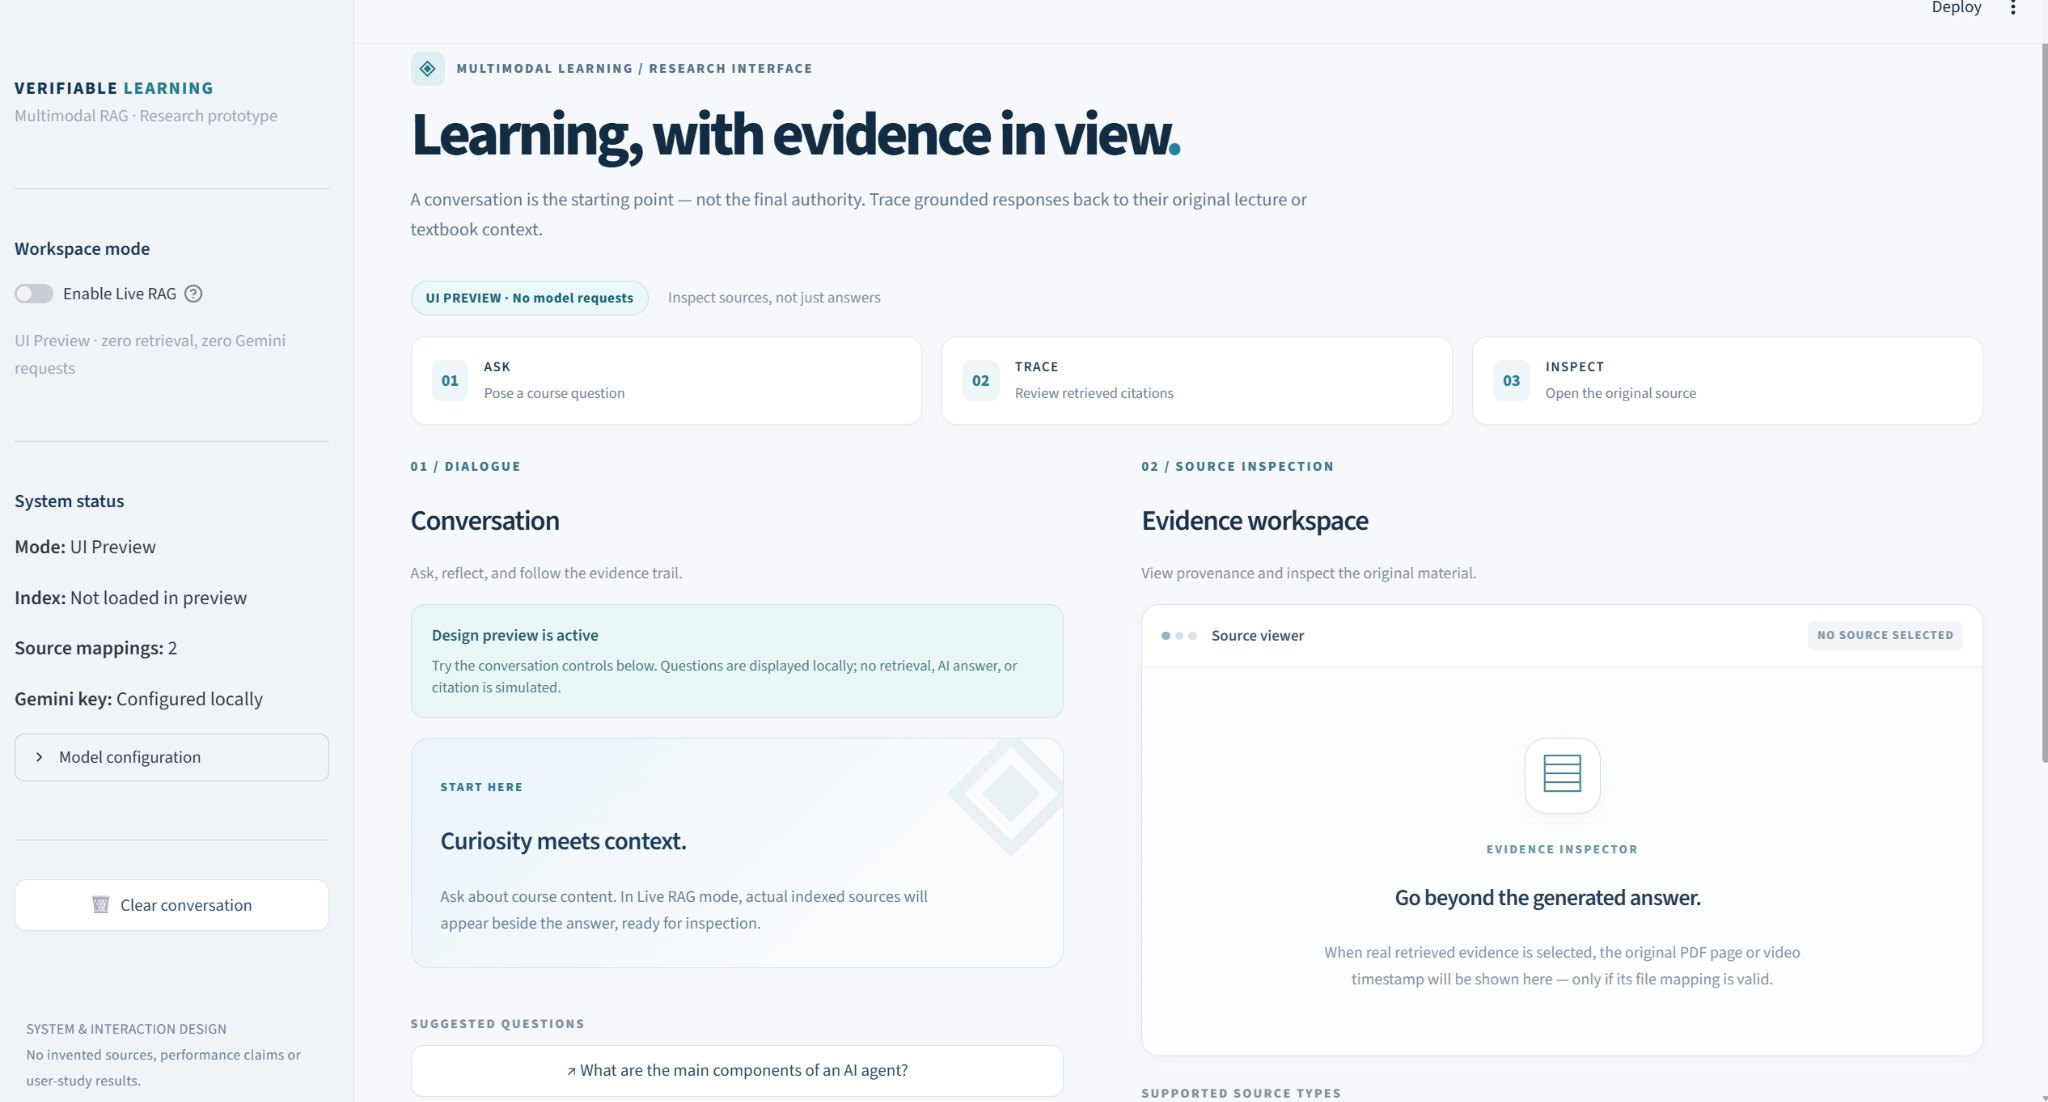
\includegraphics[width=0.97\linewidth]{ui-preview.jpg}
\Description{Real local screenshot of the redesigned light-themed Streamlit interface. A sidebar indicates UI Preview mode. The conversation panel and evidence workspace are visible, but no retrieved citation and no opened PDF or video are shown.}
\caption{Actual local screenshot of the redesigned Streamlit UI Preview. The layout and evidence-workspace empty state are visible; this image is \emph{not} evidence of successful retrieval, generated answers, video seeking, or PDF navigation.}
\label{fig:ui}
\end{figure}

\section{Implementation Evidence and Artifact Boundaries}
The public repository provides application, preprocessing, retrieval, source-mapping and viewer code, together with unit tests and documentation. The original private index contained PDF text, figure descriptions, and timestamped video-description records, and a local run displayed retrieved video-source buttons while answer generation failed with an API retry error. These observations support the existence of an indexed retrieval path and rendered evidence controls in that local environment, not general correctness or reliability claims.

\begin{table}[t]
\caption{Distinguishing implemented code from observed execution and unverified behavior at the date of this revision.}
\label{tab:status}
\small
\begin{tabularx}{\linewidth}{@{}>{\raggedright\arraybackslash}p{0.35\linewidth}X@{}}
\toprule
Capability & Status and evidential boundary \\
\midrule
Dense retrieval and node metadata & Implemented; persisted private index inspected; retrieved video controls observed locally. No retrieval-quality benchmark. \\
UI Preview and evidence layout & Implemented; real local screenshot observed; preview issues no model calls and creates no citations. \\
Source registry and validation & Implemented in Python; unit-tested for metadata and missing-source cases. \\
PDF page rendering / video start time & Viewer code present; navigation with matching original PDF/MP4 not end-to-end verified. \\
Answer generation & Gemini call path present; no reliable completed answer-generation run is asserted for this revision. \\
ASR, BM25, per-claim attribution, passage highlighting & Not implemented or not validated as a current capability. \\
\bottomrule
\end{tabularx}
\end{table}

The original teaching PDF and lecture video were obtained from third-party educational materials. The public repository therefore excludes those media, extracted pages and frames, processed content exports, and the persisted index, which could reproduce protected content. As a result, a clean public checkout supports inspecting the code and UI Preview, but it is not a turnkey end-to-end RAG reproduction. An authorized user must supply matching original media, build or privately provide an index, and configure source mappings. The original index's legacy labels also limit reliable mapping across multiple distinct documents without reindexing using stable source identifiers.

These release choices are deliberate provenance and intellectual-property constraints, not evidence that original-media navigation has succeeded. The unit tests exercise specific data and control paths rather than measuring learner behavior, model accuracy, or browser-level seeking.

\section{Illustrative Interaction and Design Analysis}
The following scenarios are conceptual walkthroughs, not reported participant sessions or measured outcomes.

\subsection{Text-Grounded Query}
A learner asks where a concept is defined in the textbook. An indexed passage may contain a page number and, if the source registry resolves to the correct edition, the interface can attempt to render that page. The learner must inspect the surrounding text to decide whether the passage supports the explanation. The design does not provide reliable passage highlighting because the legacy records lack passage geometry.

\subsection{Video-Grounded Query}
A learner asks where a lecture visually demonstrates a procedure. A timestamped frame description may retrieve a candidate moment. The interface can expose its indexed seconds as a video-source button and, when matching local media are available, request a seek to that time. A wrong caption or a mismatch between indexed timestamps and the current video remains detectable only through actual inspection, not through the citation label itself.

\subsection{Cross-Modal Query}
A learner asks how a textbook definition relates to a diagram or lecture example. Dense retrieval may return records with different source types. The interface can display their original positions side by side with the answer. It does not automatically establish a semantic relation or a sentence-level correspondence between those records; the comparison remains a task for the learner.

\section{Discussion}
\subsection{Verifiable Interaction as a Design Principle}
We define \emph{verifiable interaction} as an interface arrangement that lets a person move from an AI explanation or retrieved reference to an inspectable original source. Its immediate promise is \emph{availability of inspection}, not verified correctness. A plausible answer may cite an irrelevant source; a valid page or time coordinate may identify material that fails to support the accompanying claim. Retrieval relevance, attribution, and learner judgment remain distinct. Human--AI interaction research motivates preserving opportunities for appropriate reliance~\cite{amershi2019guidelines,holstein2020framework}.

\subsection{Temporal Coordinates as Interface Primitives}
In a video-based tutor, timestamp metadata can also become a player-control input. This connects retrieval to navigation without requiring a new retrieval algorithm. The conversion is still vulnerable to timestamp drift, mismatched video editions, clip boundaries, and unrepresentative sampled frames. More granular intervals and speech alignment could improve navigability but are future capabilities, not properties verified here.

\subsection{Inspectability Rather Than Model Explainability}
Generated explanations and external-source actions serve different epistemic functions. A rationale may sound coherent without faithfully describing model computation~\cite{miller2019explanation}. A source viewer offers something else: access to a document or recording that exists outside the answer. That access does not prove model faithfulness or that a retrieved node supports each sentence.

\subsection{Educational Implications}
Inspectable evidence may give learners the opportunity to question, compare, and revise generated guidance. It may also impose switching and reading costs; interface access does not ensure use. Cognitive-load theory~\cite{sweller2011cognitive} motivates examining these costs, but cannot by itself establish that the proposed layout reduces cognitive load. Future empirical work should distinguish source availability, successful navigation, actual inspection behavior, and educational outcomes.

\section{Limitations}
This is a system and interaction-design preprint. It does not report a controlled user study, an evaluated retrieval benchmark, validated claim attribution, or measured learning improvements. A preliminary workshop manuscript contained quantitative and participant-based claims for which sufficient supporting records were not available during this revision. Those findings and figures are excluded and do not support the present arguments.

The public code release expands the inspectable artifacts beyond the original architecture drawing and chat screenshot. Nevertheless, the protected teaching data and private index are not redistributed, and actual PDF/video click-through remains incompletely verified. The preview screenshot shows the layout only. Code-level support for viewer navigation must not be confused with a confirmed successful media-seeking session. Similarly, the current video path uses frame captions rather than speech transcription; BM25-based hybrid retrieval, precise passage highlighting, and automatic sentence-to-evidence attribution remain outside the implemented scope.

Document extraction, frame sampling, and model-generated visual descriptions can introduce errors. The legacy index does not consistently preserve stable source identifiers or image-page metadata. Even a navigable reference may point to the wrong edition, an irrelevant frame, or incomplete supporting context. Scaffolding-oriented prompting cannot guarantee appropriate pedagogy, and the effect of source inspection on learning, trust, effort, or performance remains unknown.

\section{Future Work}
A next engineering milestone is an openly redistributable, small author-created PDF/video corpus with explicitly defined source IDs and positions. It would enable reproducible tests of citation resolution and video/PDF navigation, including stale references, malformed timestamps, mismatched editions, and missing-source states. The same corpus could support comparisons of dense and lexical retrieval strategies and evaluation of whether retrieved material actually supports individual claims.

An HCI study could then compare actionable citations with static source labels, examining whether learners can reach intended sources, detect unsupported AI explanations, and use evidence during learning. Such a study would require an appropriate design, consent and relevant institutional review, with outcomes reported only after measurement.

\section{Conclusion}
We have presented a system and interface-design account of a multimodal learning prototype that connects textbook passages and timestamped lecture-frame descriptions to source-oriented interaction controls. Its distinguishing architectural choice is to keep provenance metadata separate from generated prose and to make source resolution an explicit, failure-aware interface operation. The public code artifact makes this choice inspectable while clearly separating implementation from unverified end-to-end behavior. We refer to this design objective as \emph{verifiable interaction}; it offers a path to source inspection, not an automatic guarantee of factual accuracy, trust, or learning benefit.

% References carried over from the supplied manuscript without inventing citations.
\begin{thebibliography}{99}

\bibitem{sweller2011cognitive}
J. Sweller, P. Ayres, and S. Kalyuga.
\newblock \emph{Cognitive Load Theory}.
\newblock Springer, 2011.
\newblock
\url{https://doi.org/10.1007/978-1-4419-8126-4}.

\bibitem{mayer2020multimedia}
R. E. Mayer.
\newblock \emph{Multimedia Learning}, 3rd ed.
\newblock Cambridge University Press, 2020.
\newblock
\url{https://www.cambridge.org/highereducation/books/multimedia-learning/FB7E79A165D24D47CEACEB4D2C426ECD}.

\bibitem{lewis2020rag}
P. Lewis, E. Perez, A. Piktus, F. Petroni,
V. Karpukhin, N. Goyal, H. K\"uttler,
M. Lewis, W.-t. Yih, T. Rockt\"aschel,
S. Riedel, and D. Kiela.
\newblock Retrieval-augmented generation for
knowledge-intensive NLP tasks.
\newblock In \emph{Advances in Neural Information
Processing Systems}, vol.~33,
pp.~9459--9474, 2020.
\newblock
\url{https://proceedings.neurips.cc/paper/2020/hash/6b493230205f780e1bc26945df7481e5-Abstract.html}.

\bibitem{sperber2010vigilance}
D. Sperber, F. Cl\'ement, C. Heintz,
O. Mascaro, H. Mercier, G. Origgi,
and D. Wilson.
\newblock Epistemic vigilance.
\newblock \emph{Mind \& Language},
25(4):359--393, 2010.
\newblock
\url{https://doi.org/10.1111/j.1468-0017.2010.01394.x}.

\bibitem{zimmerman2002self}
B. J. Zimmerman.
\newblock Becoming a self-regulated learner:
An overview.
\newblock \emph{Theory Into Practice},
41(2):64--70, 2002.
\newblock
\url{https://doi.org/10.1207/s15430421tip4102_2}.

\bibitem{amershi2019guidelines}
S. Amershi, D. Weld, M. Vorvoreanu,
A. Fourney, B. Nushi, P. Collisson,
J. Suh, S. Iqbal, P. N. Bennett,
K. Inkpen, J. Teevan, R. Kikin-Gil,
and E. Horvitz.
\newblock Guidelines for human--AI interaction.
\newblock In \emph{Proceedings of CHI 2019},
Article~3, pp.~1--13, 2019.
\newblock
\url{https://doi.org/10.1145/3290605.3300233}.

\bibitem{miller2019explanation}
T. Miller.
\newblock Explanation in artificial intelligence:
Insights from the social sciences.
\newblock \emph{Artificial Intelligence},
267:1--38, 2019.
\newblock
\url{https://doi.org/10.1016/j.artint.2018.07.007}.

\bibitem{zhong2022video}
Y. Zhong, W. Ji, J. Xiao, Y. Li,
W. Deng, and T.-S. Chua.
\newblock Video question answering:
Datasets, algorithms and challenges.
\newblock In \emph{Proceedings of EMNLP 2022},
pp.~6439--6455, 2022.
\newblock
\url{https://doi.org/10.18653/v1/2022.emnlp-main.432}.

\bibitem{zhao2025mdkag}
X. Zhao, G. Wang, and Y. Lu.
\newblock MDKAG: Retrieval-augmented
educational QA powered by a multimodal
disciplinary knowledge graph.
\newblock \emph{Applied Sciences},
15(16):9095, 2025.
\newblock
\url{https://doi.org/10.3390/app15169095}.

\bibitem{hu2025mrag}
C.-W. Hu, Y. Wang, S. Xing, C.-J. Chen,
S. Feng, R. Rossi, and Z. Tu.
\newblock mRAG: Elucidating the design space
of multi-modal retrieval-augmented generation.
\newblock \emph{arXiv preprint}
arXiv:2505.24073, 2025.
\newblock
\url{https://arxiv.org/abs/2505.24073}.

\bibitem{delarosa2025video}
K. Dela Rosa.
\newblock Video-enriched retrieval augmented
generation using aligned video captions.
\newblock In \emph{Companion Proceedings of the
ACM Web Conference 2025 (WWW Companion '25)},
pp.~1663--1667, 2025.
\newblock
\url{https://doi.org/10.1145/3701716.3716890}.

\bibitem{cuconasu2024noise}
F. Cuconasu, G. Trappolini, F. Siciliano,
S. Filice, C. Campagnano, Y. Maarek,
N. Tonellotto, and F. Silvestri.
\newblock The power of noise:
Redefining retrieval for RAG systems.
\newblock In \emph{Proceedings of SIGIR 2024},
pp.~719--729, 2024.
\newblock
\url{https://doi.org/10.1145/3626772.3657834}.

\bibitem{holstein2020framework}
K. Holstein, V. Aleven, and N. Rummel.
\newblock A conceptual framework for human--AI
hybrid adaptivity in education.
\newblock In \emph{Artificial Intelligence
in Education (AIED 2020)},
Lecture Notes in Computer Science,
vol.~12163, pp.~240--254.
Springer, 2020.
\newblock
\url{https://doi.org/10.1007/978-3-030-52237-7_20}.

\bibitem{kasneci2023chatgpt}
E. Kasneci, K. Se\ss{}ler, S. K\"uchemann,
M. Bannert, D. Dementieva, F. Fischer, et al.
\newblock ChatGPT for good? On opportunities
and challenges of large language models
for education.
\newblock \emph{Learning and Individual
Differences}, 103:102274, 2023.
\newblock
\url{https://doi.org/10.1016/j.lindif.2023.102274}.

\end{thebibliography}
\end{document}
